\documentclass[border=10pt]{standalone}
\usepackage{circuitikz}
\usepackage{tikz}
\usetikzlibrary{calc}

\begin{document}
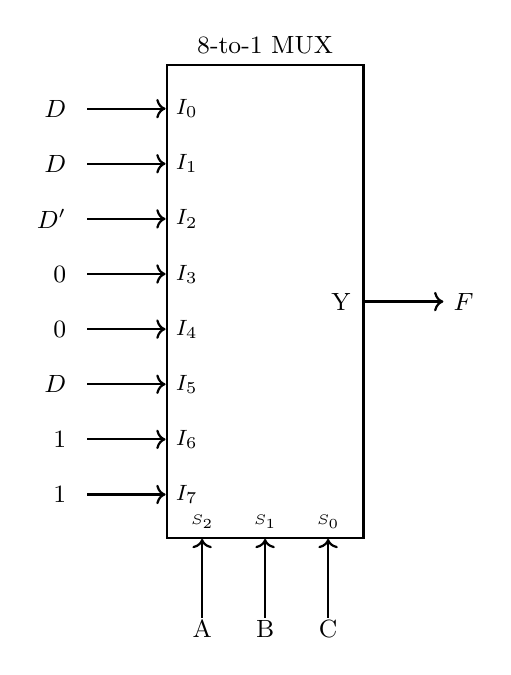
\begin{tikzpicture}[
    thick,
    font=\small,
    mux/.style={draw, rectangle, minimum width=2.5cm, minimum height=6cm}
]

    % MUX Block
    \node[mux] (M) at (0, 0) {};
    \node[above] at (M.north) {8-to-1 MUX};
    \node at ($(M.east) + (-0.3, 0)$) {Y};
    
    % Select Inputs
    \draw[<-] ($(M.south) + (-0.8, 0)$) -- ++(0, -1) node[above,font=\tiny][yshift=+1cm] {$S_2$};
    \draw[<-] ($(M.south) + (0, 0)$) -- ++(0, -1) node[above,font=\tiny][yshift=+1cm] {$S_1$};
    \draw[<-] ($(M.south) + (0.8, 0)$) -- ++(0, -1) node[above,font=\tiny][yshift=+1cm] {$S_0$};
    
    % Variable labels for Selects
    %\node[below=0.6cm] at ($(M.south) + (-0.8, 0)$) {$\uparrow$};
    \node[below=0.9cm] at ($(M.south) + (-0.8, 0)$) {A};
    
    %\node[below=0.6cm] at ($(M.south) + (0, 0)$) {$\uparrow$};
    \node[below=0.9cm] at ($(M.south) + (0, 0)$) {B};

    %\node[below=0.6cm] at ($(M.south) + (0.8, 0)$) {$\uparrow$};
    \node[below=0.9cm] at ($(M.south) + (0.8, 0)$) {C};

    % Output
    \draw[->] (M.east) -- ++(1, 0) node[right] {$F$};

    % Data Inputs (I0 to I7)
    \foreach \i in {0,...,7} {
        % Calculate vertical position. Top is roughly +2.5, Bottom -2.5
        % spacing = 5 / 7 approx 0.7
        \coordinate (input\i) at ($(M.west) + (0, {2.45 - \i*0.7})$);
        \draw[<-] (input\i) -- ++(-1, 0) node[left] (node\i) {};
        \node[right, font=\footnotesize] at (input\i) {$I_{\i}$};
    }

    % Derived Logic Inputs based on F = Sum(1, 3, 4, 11, 12, 13, 14, 15)
    % Pairs: (0,1), (2,3), (4,5), (6,7), (8,9), (10,11), (12,13), (14,15)
    % Terms: D' D   D' D   D' D   D' D   D' D   D' D     D' D     D' D
    % I0 (0,1 -> 1): F=D
    % I1 (2,3 -> 3): F=D
    % I2 (4,5 -> 4): F=D'
    % I3 (6,7 -> X): F=0
    % I4 (8,9 -> X): F=0
    % I5 (10,11 -> 11): F=D
    % I6 (12,13 -> 12,13): F=1
    % I7 (14,15 -> 14,15): F=1

    % Let's verify:
    % 0 (0000): 0 -> D' (0)
    % 1 (0001): 1 -> D (1) -> I0 = D
    
    % 2 (0010): 0 -> D' (0)
    % 3 (0011): 1 -> D (1) -> I1 = D
    
    % 4 (0100): 1 -> D' (1)
    % 5 (0101): 0 -> D (0) -> I2 = D'
    
    % 6 (0110): 0 -> D' (0)
    % 7 (0111): 0 -> D (0) -> I3 = 0
    
    % 8 (1000): 0 -> D' (0)
    % 9 (1001): 0 -> D (0) -> I4 = 0
    
    % 10 (1010): 0 -> D' (0)
    % 11 (1011): 1 -> D (1) -> I5 = D
    
    % 12 (1100): 1 -> D' (1)
    % 13 (1101): 1 -> D (1) -> I6 = 1
    
    % 14 (1110): 1 -> D' (1)
    % 15 (1111): 1 -> D (1) -> I7 = 1
    
    % Values: D, D, D', 0, 0, D, 1, 1
    
    \node[left] at (node0) {$D$};
    \node[left] at (node1) {$D$};
    \node[left] at (node2) {$D'$};
    \node[left] at (node3) {$0$};
    \node[left] at (node4) {$0$};
    \node[left] at (node5) {$D$};
    \node[left] at (node6) {$1$};
    \node[left] at (node7) {$1$};

\end{tikzpicture}
\end{document}
